% ============================================================================
%  HI-VQE on Li2S at 24 Qubits
%  A variationally bounded method as a certificate on its own reference
%
%  Compile:  pdflatex main.tex     (run three times: ToC + cross-references)
%  No bibtex pass required -- the bibliography is inline.
%  Figures expected in ./figures/
% ============================================================================
\documentclass[11pt,a4paper]{article}

\usepackage[T1]{fontenc}
\usepackage[utf8]{inputenc}
\usepackage{lmodern}
\usepackage[margin=2.4cm,headheight=14pt]{geometry}
\usepackage{amsmath,amssymb}
\usepackage{graphicx}
\usepackage{booktabs}
\usepackage{array}
\usepackage{caption}
\usepackage{enumitem}
\usepackage{fancyhdr}
\usepackage{microtype}
\usepackage{xcolor}

\definecolor{NavyLink}{HTML}{1A4C8B}
\definecolor{BoxBlue}{HTML}{EAF1F9}
\definecolor{BoxRule}{HTML}{1A4C8B}
\definecolor{WarnBg}{HTML}{FDF3E7}
\definecolor{WarnRule}{HTML}{9C5B12}
\definecolor{StopBg}{HTML}{F5EEEE}
\definecolor{StopRule}{HTML}{8B1A1A}

\usepackage{tcolorbox}
\usepackage[colorlinks=true,linkcolor=NavyLink,citecolor=NavyLink,
            urlcolor=NavyLink,bookmarksnumbered=true]{hyperref}

\newtcolorbox{result}[1][]{%
  colback=BoxBlue, colframe=BoxRule, boxrule=0.7pt, arc=1.5pt,
  left=6pt, right=6pt, top=5pt, bottom=5pt,
  fonttitle=\bfseries\sffamily\small, title={#1}}

\newtcolorbox{caution}[1][]{%
  colback=WarnBg, colframe=WarnRule, boxrule=0.7pt, arc=1.5pt,
  left=6pt, right=6pt, top=5pt, bottom=5pt,
  fonttitle=\bfseries\sffamily\small, title={#1}}

\newtcolorbox{unsupported}[1][]{%
  colback=StopBg, colframe=StopRule, boxrule=0.7pt, arc=1.5pt,
  left=6pt, right=6pt, top=5pt, bottom=5pt,
  fonttitle=\bfseries\sffamily\small, title={#1}}

\pagestyle{fancy}
\fancyhf{}
\fancyhead[L]{\small\itshape HI-VQE on Li$_2$S at 24 qubits}
\fancyhead[R]{\small\thepage}
\renewcommand{\headrulewidth}{0.4pt}

\captionsetup{font=small,labelfont=bf,skip=6pt}
\setlength{\parskip}{0.30em}
\setlength{\parindent}{0pt}

\renewcommand{\topfraction}{0.92}
\renewcommand{\bottomfraction}{0.75}
\renewcommand{\textfraction}{0.06}
\renewcommand{\floatpagefraction}{0.75}
\setcounter{topnumber}{3}
\setcounter{bottomnumber}{2}
\setcounter{totalnumber}{5}
\raggedbottom

% Long \code{} identifiers are unbreakable; give TeX slack rather than
% hyphenating typewriter text or shortening the identifiers themselves.
\setlength{\emergencystretch}{3em}

\newcommand{\mHa}{\ensuremath{\,\mathrm{mHa}}}
\newcommand{\Ha}{\ensuremath{\,\mathrm{Ha}}}
\newcommand{\Ang}{\ensuremath{\,\text{\AA}}}
\newcommand{\Ssq}{\ensuremath{\langle \hat{S}^2 \rangle}}
\newcommand{\code}[1]{\texttt{\small #1}}
\newcommand{\LiS}{\texorpdfstring{Li$_2$S}{Li2S}}

\title{\vspace{-1.1cm}\textbf{HI-VQE on Li$_2$S at 24 Qubits}\\[0.4em]
\large A variationally bounded method used as a\\
certificate on its own reference}
\author{Bhargav Krishna\\\small\texttt{qacd@qimlabs.com}}
\date{\today}

\begin{document}
\maketitle
\thispagestyle{fancy}

\begin{abstract}
\noindent
The Handover Iterative Variational Quantum Eigensolver (HI-VQE, Pellow-Jarman
\emph{et al.}, arXiv:2503.06292) is implemented on Qiskit and applied to that
paper's own benchmark system: Li$_2$S in CAS(12e,12o)/STO-3G, 24 qubits,
$853{,}776$ determinants, along the Li--S dissociation coordinate. Thirteen
geometries were computed, together with a classical selected-CI control, an
ablation of the algorithm's two halves, and MP2/CCSD/CCSD(T) baselines in the
identical active space.

Eleven of thirteen geometries land inside chemical accuracy of exact
diagonalisation, at a mean error of $0.081\mHa$ over those points, using a mean
of $2.25\%$ of the determinant space. Hartree--Fock misses the same curve by up
to $168\mHa$. The dissociation energy computed from the curve is $103.89$
kcal/mol against exact diagonalisation's $103.94$ --- an error of $0.051$
kcal/mol --- and because a dissociation energy is a difference, that is a
stricter consistency test than any single total energy. The sampling circuit
requires one measurement setting where a conventional VQE on this Hamiltonian
would require $15{,}697$ Pauli words per optimiser step.

The two geometries that fail do so in a way worth reporting. At $3.20$ and
$3.60\Ang$ the HI-VQE energy lies \emph{below} the CASCI reference, by $8.50$
and $24.24\mHa$. For a variational method whose energy is the lowest eigenvalue
of $PHP$ for a projector $P$, that is impossible against a correct reference ---
so the finding is not that HI-VQE erred, but that the reference at those two
points is not the ground state of the sector it was intended to diagonalise. Two
independent arguments confirm this: the variational bound itself, and the
non-monotonicity it induces in the reference potential-energy curve. Both
failing points return $\Ssq = 2.00$, the triplet.

The ablation is reported with its negative reading intact: a classical
selected-CI control with no circuit at all reaches $0.141\mHa$ at the
equilibrium geometry, against the quantum-sampled $0.076\mHa$. At this size the
classical expansion is sufficient, and the table exists so that the statement is
checkable rather than assumed.
\end{abstract}

\tableofcontents
\vspace{0.6em}
\hrule
\vspace{0.8em}

\section{Introduction}

\subsection{What HI-VQE changes}

A conventional VQE asks a quantum device for an \emph{energy}. That requires
measuring every Pauli word in the Hamiltonian, every iteration. For this system
the published work counts $15{,}697$ Pauli words --- $15{,}697$ measurement
settings per optimiser step --- and \code{run.py paulis} recomputes that figure
from the cached integrals, so it is checkable rather than quoted.

HI-VQE asks a different question: \emph{which electron configurations matter?}
One measurement of the sampling circuit returns a set of occupation bitstrings.
The Hamiltonian is projected onto the subspace those configurations span and
diagonalised exactly, classically. That is the handover.

\begin{table}[htbp]
\centering
\caption{Three consequences of the handover, and where each is checked in this
implementation rather than asserted.}
\label{tab:consequences}
\small
\begin{tabular}{>{\raggedright\arraybackslash}p{0.26\textwidth}>{\raggedright\arraybackslash}p{0.34\textwidth}>{\raggedright\arraybackslash}p{0.32\textwidth}}
\toprule
Property & Why it follows & Where it is checked \\
\midrule
The energy is a strict upper bound &
$PHP$ has its lowest eigenvalue above the true ground state for \emph{any}
projector $P$, so device noise can worsen the subspace but never push the energy
below the answer &
\code{validate} on random subspaces; any violation is reported as
\code{INCONSISTENT} and never as a result \\
\addlinespace
The energy is monotone in the subspace &
the subspace only grows &
\code{history} in every result file, and a re-solve guard inside the loop \\
\addlinespace
The quantum layer is separable &
\code{--simulator none} removes it entirely; \code{--no-expansion} removes the
classical half instead &
the ablation table, \S\ref{sec:ablation} \\
\bottomrule
\end{tabular}
\end{table}

The third row is the honest one, and it frames this entire report. At 24 qubits
the full CAS space is $853{,}776$ determinants, which a laptop diagonalises
directly. This is therefore a \textbf{benchmark and validation exercise, not a
claim of quantum advantage}, and the ablation exists precisely so that the
quantum layer's contribution is a number the reader inspects rather than a claim
the reader accepts.

\subsection{System and active space}

Li$_2$S has 22 electrons in STO-3G. CAS(12e,12o) freezes the five lowest
orbitals --- the sulfur $1s$, $2s$ and $2p$ shell, which sit near $-91$, $-9$
and $-6.7\Ha$ while nothing else in the molecule lies below $-3\Ha$ --- and
drops the two highest virtuals. \code{prepare} measures this rather than
assuming it and refuses to build if the frozen orbitals are not the sulfur
core; the recorded core--active gap is $3.89\Ha$.

\begin{table}[htbp]
\centering
\caption{The system and the resulting qubit problem.}
\label{tab:system}
\small
\begin{tabular}{ll}
\toprule
Geometry            & linear Li--S--Li, one bond stretched \\
Basis               & STO-3G \\
Orbitals            & canonical RHF \\
Frozen core         & 5 orbitals, core--active gap $3.89\Ha$ \\
Active space        & CAS(12e,12o) \\
Qubits              & $24$ \\
Full CAS dimension  & $853{,}776$ determinants \\
Reference           & CASCI, exact within the active space \\
Coordinate          & 13 geometries, $1.70$ to $6.00\Ang$ \\
\bottomrule
\end{tabular}
\end{table}

\subsection{Scope and claims}

\begin{enumerate}[leftmargin=1.4em,itemsep=0.15em]
\item HI-VQE reproduces exact diagonalisation to better than $0.15\mHa$ at
  eleven of thirteen geometries, sampling ${\sim}2.3\%$ of the determinant
  space.
\item The dissociation energy derived from that curve is within $0.051$
  kcal/mol of the exact one.
\item At two geometries the reference itself is invalid, and the variational
  bound of the method is what establishes this.
\item The classical baselines fail beyond $4.20\Ang$ for a reason that is
  diagnosable from the $T_1$ amplitude, and this is why CASCI rather than
  CCSD(T) is the reference.
\item The quantum sampler's contribution at this size is a better \emph{starting}
  subspace, not a better final energy.
\end{enumerate}

\section{Method}

\subsection{The sampling circuit}

A hardware-efficient unitary cluster Jastrow, built as a real Qiskit circuit:

\begin{itemize}[leftmargin=1.4em,itemsep=0.15em]
\item nearest-neighbour Givens rotations (\code{XXPlusYY}) in a brickwork of
  depth $M$ inside each spin block. Depth $M$ is what the Clements decomposition
  requires to realise an arbitrary orbital rotation, so one network can move an
  electron from any orbital to any other. A shallower network cannot, and the
  proposal distribution collapses onto Hartree--Fock and its immediate
  neighbours;
\item a diagonal number--number Jastrow layer (\code{RZ}, \code{RZZ}), including
  the same-orbital $\alpha$--$\beta$ terms, which are the only gates correlating
  the two spin blocks;
\item \textbf{a closing Givens network, never a closing Jastrow layer.} A
  trailing diagonal layer changes only phases, so it is exactly invisible to a
  measurement distribution --- it would cost gates and shots while doing
  nothing. The self-test checks that claim rather than trusting it.
\end{itemize}

Every gate commutes with the $\alpha$ and $\beta$ number operators separately.
On a noiseless simulator, therefore, \textbf{every shot is a valid
configuration}: no electron-count filtering, no wasted shots, leakage exactly
zero rather than merely small. At all-zero angles the circuit is exactly the
Hartree--Fock determinant.

\begin{table}[htbp]
\centering
\caption{Circuit resources at 24 qubits, as recorded in every result file.}
\label{tab:circuit}
\small
\begin{tabular}{lr}
\toprule
Qubits                     & $24$ \\
Depth                      & $29$ \\
Circuit size               & $334$ \\
Two-qubit gates            & $298$ \\
Parameters                 & $322$ \\
Transpiled depth, linear chain & $451$ \\
Transpiled two-qubit gates (CZ) & $992$ \\
Basis                      & \code{rz, sx, x, cz} \\
\bottomrule
\end{tabular}
\end{table}

\begin{figure}[htbp]
\centering
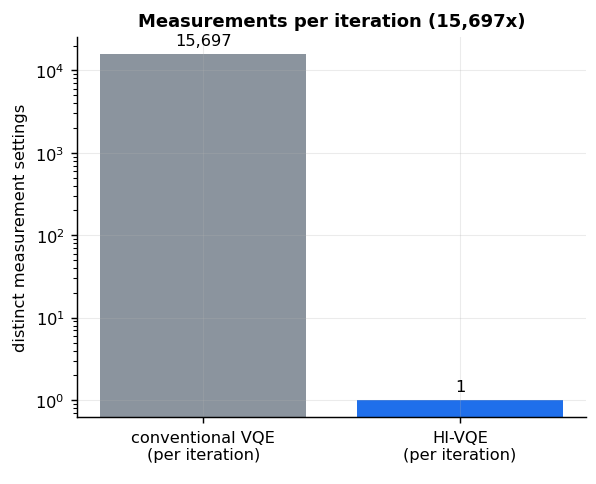
\includegraphics[width=0.56\textwidth]{figures/b-cost-measurement.png}
\caption{Measurement settings per iteration: $15{,}697$ Pauli words for a
conventional VQE on this Hamiltonian against one for HI-VQE, drawn to scale.
This is the resource claim the method rests on.}
\label{fig:costmeas}
\end{figure}

\begin{figure}[htbp]
\centering
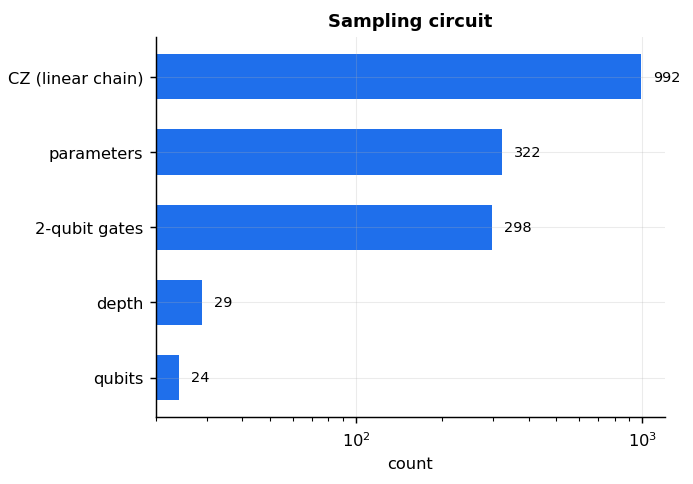
\includegraphics[width=0.62\textwidth]{figures/b-cost-circuit.png}
\caption{The sampling circuit's own gate counts, before and after transpilation
to a linear chain.}
\label{fig:costcirc}
\end{figure}

\subsection{The two simulators}

\begin{table}[htbp]
\centering
\caption{Simulator options. \code{sector} is the working default; \code{aer} is
the reference path and the only one that can carry a noise model.}
\label{tab:sims}
\small
\begin{tabular}{>{\raggedright\arraybackslash}p{0.20\textwidth}>{\raggedright\arraybackslash}p{0.24\textwidth}>{\raggedright\arraybackslash}p{0.22\textwidth}>{\raggedright\arraybackslash}p{0.22\textwidth}}
\toprule
& \code{sector} (default) & \code{aer} & \code{none} \\
\midrule
What it is & exact statevector inside the $853{,}776$-dimensional
particle-number sector & Qiskit Aer over all $16{,}777{,}216$ amplitudes & no
quantum layer at all \\
\addlinespace
Cost per sample & ${\sim}2.8$ s & ${\sim}11$ s & $0$ \\
Noise models & no --- noiseless by construction & \textbf{yes} & --- \\
Role & the working default & the reference path & classical control \\
\bottomrule
\end{tabular}
\end{table}

\code{sector\_sim.py} is fast because the ansatz never leaves the sector, and it
is trustworthy because it \textbf{reimplements nothing}: it reads each gate's own
\code{to\_matrix()} from the Qiskit circuit and applies that, so Qiskit remains
the sole authority on what \code{XXPlusYY}$(\theta)$ means.
\code{run.py backend --full} cross-checks the two amplitude by amplitude on the
real 24-qubit circuit; the self-test does the same on a small one.

\subsection{Acceptance criteria}
\label{sec:criteria}

\begin{table}[htbp]
\centering
\caption{Verdicts, and what each one means. \code{INCONSISTENT} is the one that
matters for \S\ref{sec:invalid}.}
\label{tab:verdicts}
\small
\begin{tabular}{>{\raggedright\arraybackslash}p{0.28\textwidth}>{\raggedright\arraybackslash}p{0.66\textwidth}}
\toprule
Verdict & Meaning \\
\midrule
\code{CHEMICAL ACCURACY} & within $1.6\mHa$ of CASCI, above it, and a spin
eigenstate \\
\code{OUTSIDE CHEMICAL ACCURACY} & working but subspace-limited; raise
\code{--max-determinants} or \code{--expansion} \\
\code{INCONSISTENT} & \textbf{below} CASCI --- impossible for a projected
subspace. Re-run \code{validate} and \code{selftest}; do not report the number \\
\code{SPIN CONTAMINATED} & $\Ssq$ is not near any $S(S+1)$, so the subspace is
not spin-complete \\
\code{PT2 IS NOT USABLE HERE} & not a verdict on the energy --- the
\emph{correction} exceeds half the correlation the subspace captured, so
perturbation theory is out of its domain \\
\bottomrule
\end{tabular}
\end{table}

Note what \code{SPIN CONTAMINATED} is \emph{not}. It does not fire on a triplet.
At a dissociated Li--S bond the singlet and triplet are nearly degenerate and
CASCI returns whichever is lower, so a triplet ground state is a result. What is
a broken calculation is a state that is neither --- and the check measures the
distance from $\Ssq$ to the nearest $S(S+1)$, not to zero.

\section{Results}

\subsection{The dissociation curve}

\begin{table}[htbp]
\centering
\caption{Thirteen geometries. One Li--S bond stretched, the other held at
equilibrium. Errors are against CASCI in the same active space; negative errors
are the subject of \S\ref{sec:invalid}.}
\label{tab:curve}
\small
\begin{tabular}{rrrrrrrr}
\toprule
$r$ (\AA) & $E$(HF) & $E$(HI-VQE) & $E$(CASCI) & err (mHa) & HF err (mHa) & dets & \% space \\
\midrule
$1.700$ & $-407.950117$ & $-407.985509$ & $-407.985607$ & $+0.0985$ & $35.5$ & $19{,}992$ & $2.342$ \\
$1.900$ & $-407.964402$ & $-408.001987$ & $-408.002076$ & $+0.0893$ & $37.7$ & $19{,}950$ & $2.337$ \\
$2.000$ & $-407.960694$ & $-407.999205$ & $-407.999309$ & $+0.1039$ & $38.6$ & $19{,}992$ & $2.342$ \\
$2.100$ & $-407.952748$ & $-407.992132$ & $-407.992208$ & $+0.0762$ & $39.5$ & $19{,}932$ & $2.335$ \\
$2.200$ & $-407.942002$ & $-407.982123$ & $-407.982225$ & $+0.1017$ & $40.2$ & $19{,}966$ & $2.339$ \\
$2.400$ & $-407.915865$ & $-407.957314$ & $-407.957425$ & $+0.1110$ & $41.6$ & $19{,}881$ & $2.329$ \\
$2.600$ & $-407.887294$ & $-407.929953$ & $-407.930087$ & $+0.1336$ & $42.8$ & $19{,}881$ & $2.329$ \\
$2.900$ & $-407.844982$ & $-407.884942$ & $-407.885013$ & $+0.0709$ & $40.0$ & $19{,}880$ & $2.328$ \\
$3.200$ & $-407.806559$ & $-407.862021$ & $-407.853522$ & $\mathbf{-8.4987}$ & $47.0$ & $19{,}881$ & $2.329$ \\
$3.600$ & $-407.764023$ & $-407.849591$ & $-407.825353$ & $\mathbf{-24.2376}$ & $61.3$ & $19{,}881$ & $2.329$ \\
$4.200$ & $-407.719485$ & $-407.840669$ & $-407.840733$ & $+0.0645$ & $121.2$ & $19{,}881$ & $2.329$ \\
$5.000$ & $-407.686955$ & $-407.837262$ & $-407.837292$ & $+0.0297$ & $150.3$ & $19{,}880$ & $2.328$ \\
$6.000$ & $-407.668269$ & $-407.836424$ & $-407.836433$ & $+0.0087$ & $168.2$ & $11{,}118$ & $1.302$ \\
\bottomrule
\end{tabular}
\end{table}

\begin{figure}[htbp]
\centering
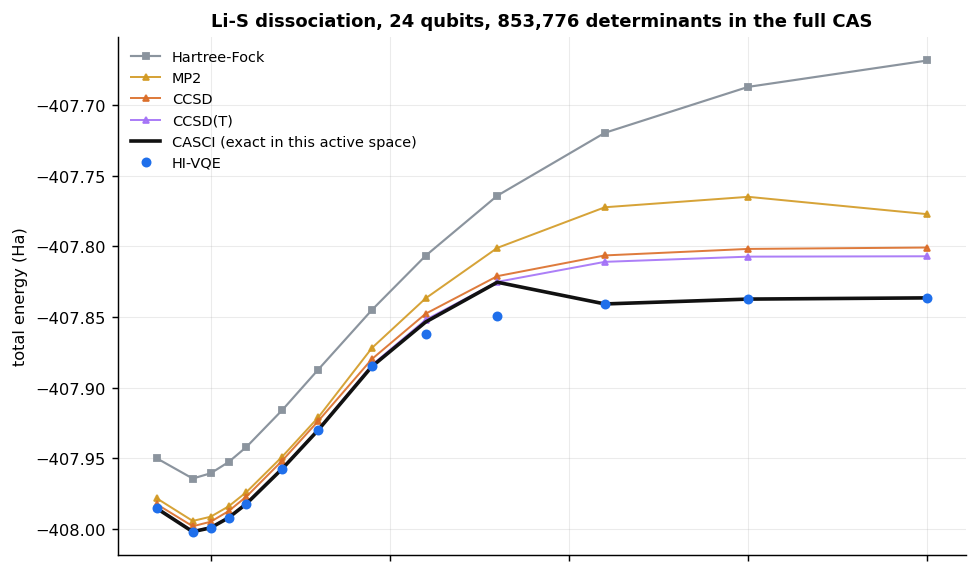
\includegraphics[width=0.76\textwidth]{figures/b-curve.png}
\caption{The dissociation curve. HI-VQE tracks CASCI everywhere the reference is
valid; Hartree--Fock's failure at long range is drawn on the same axes and is
the multireference character the method exists to capture.}
\label{fig:curve}
\end{figure}

\begin{figure}[htbp]
\centering
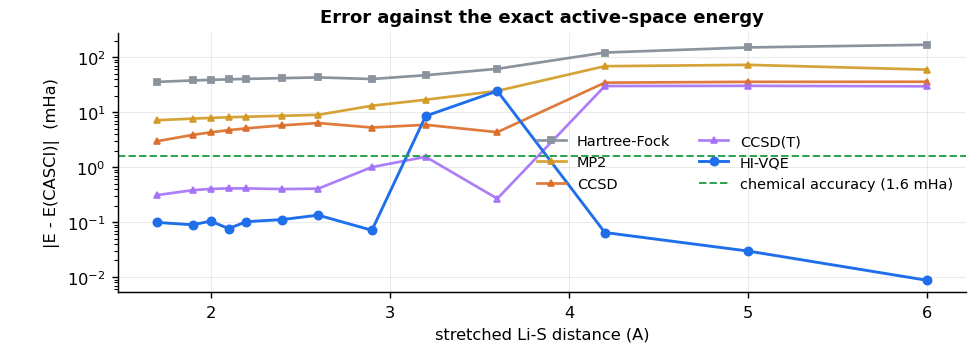
\includegraphics[width=0.76\textwidth]{figures/b-curve-error.png}
\caption{Error against CASCI on a logarithmic axis. The eleven valid points sit
between $0.009$ and $0.134\mHa$; the two excursions at $3.20$ and $3.60\Ang$ are
of the opposite sign and are analysed in \S\ref{sec:invalid}.}
\label{fig:curveerr}
\end{figure}

\begin{result}[Headline]
Across thirteen geometries: worst error $24.238\mHa$, mean $2.586\mHa$; over the
eleven valid points, all errors are below $0.135\mHa$. Hartree--Fock's error over
the same curve reaches $168.2\mHa$ with a mean of $66.5\mHa$. The mean subspace
is $19{,}239$ determinants, $2.25\%$ of the space.
\end{result}

\begin{table}[htbp]
\centering
\caption{Quantities derived from the curve. A dissociation energy is a
\emph{difference}, so the systematic part of the error cancels --- this is a
stricter test of consistency than any single total energy, and it is the number
to quote.}
\label{tab:derived}
\small
\begin{tabular}{lrr}
\toprule
Quantity & HI-VQE & CASCI \\
\midrule
Minimum on this grid & $1.900\Ang$ & $1.900\Ang$ \\
Dissociation energy to the last point & $103.89$ kcal/mol & $103.94$ kcal/mol \\
Error in that dissociation energy & $\mathbf{0.051}$ kcal/mol & --- \\
\bottomrule
\end{tabular}
\end{table}

\subsection{Convergence and compression}

\begin{figure}[htbp]
\centering
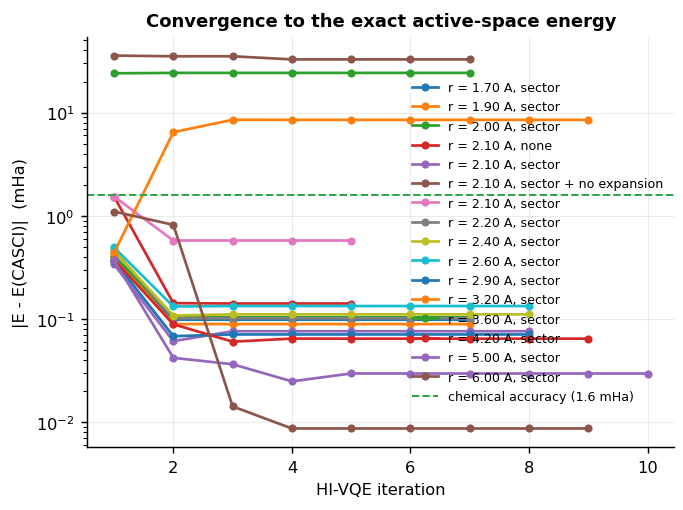
\includegraphics[width=0.62\textwidth]{figures/b-conv-error.png}
\caption{Error by iteration at the equilibrium geometry. Convergence is
monotone, as the growing-subspace argument of Table~\ref{tab:consequences}
requires.}
\label{fig:converr}
\end{figure}

\begin{figure}[htbp]
\centering
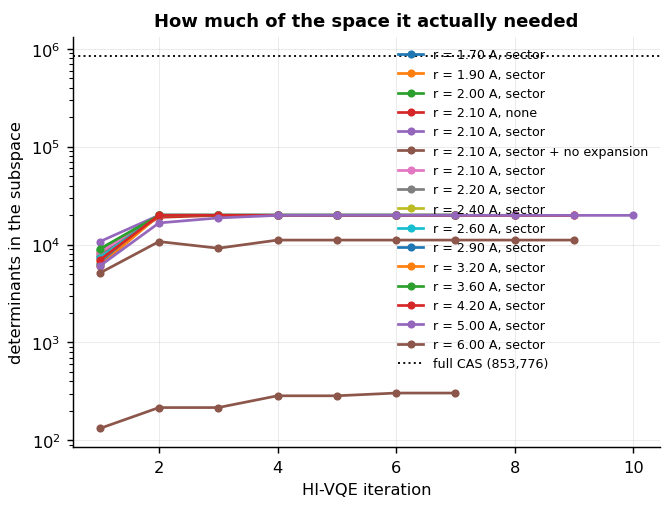
\includegraphics[width=0.62\textwidth]{figures/b-conv-dets.png}
\caption{Subspace size by iteration. The run at $2.10\Ang$ terminates after
eight iterations on the energy-tolerance criterion, holding $19{,}932$
determinants.}
\label{fig:convdets}
\end{figure}

A representative single point, $r = 2.10\Ang$: energy $-407.992132303\Ha$
against a reference of $-407.992208472\Ha$, an error of $0.0762\mHa$; $19{,}932$
determinants, $2.335\%$ of the space; $99.81\%$ of the correlation energy
recovered; $\Ssq = 1.06\times10^{-4}$; eight iterations in $67.5$ seconds;
stopped because the energy moved less than $10^{-6}\Ha$ for five consecutive
iterations. The second-order perturbative correction over $59{,}796$ additional
determinants tightens this to $0.0292\mHa$ and is flagged reliable.

\begin{figure}[htbp]
\centering
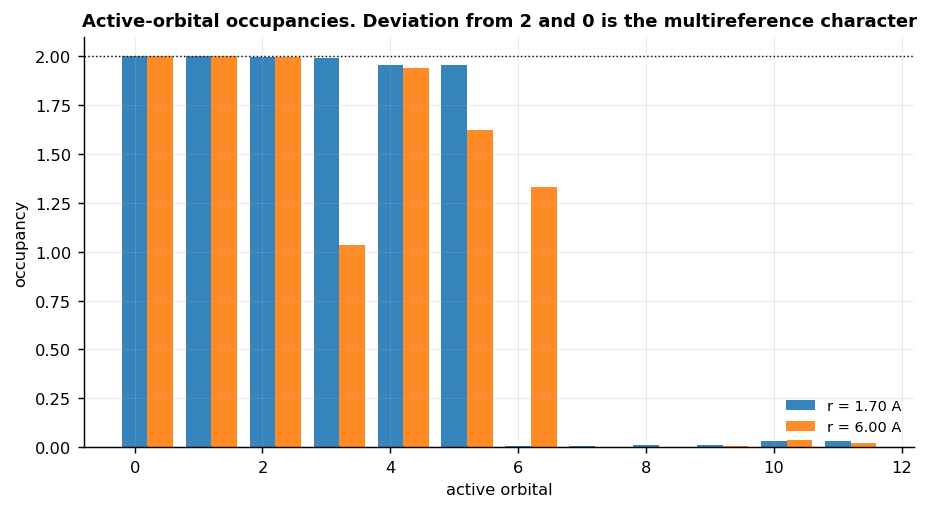
\includegraphics[width=0.70\textwidth]{figures/li2s-occupancies.png}
\caption{Natural occupancies at both ends of the coordinate. Departure from
$2$ and $0$ is the multireference character made visible, and it is what a
single-determinant reference cannot represent.}
\label{fig:occ}
\end{figure}

\subsection{Two geometries where the reference is invalid}
\label{sec:invalid}

At $3.20$ and $3.60\Ang$ the HI-VQE energy lies below the CASCI reference by
$8.50$ and $24.24\mHa$ respectively. Both runs are reported as
\code{INCONSISTENT} and neither energy is claimed as a result.

\begin{unsupported}[Why this cannot be an HI-VQE error]
The HI-VQE energy is the lowest eigenvalue of $PHP$ for a projector $P$ onto a
subspace of determinants. For \emph{any} such $P$, that eigenvalue is bounded
below by the true ground-state energy of $H$ in the sector. A projected subspace
cannot produce an energy below a correct reference --- not through a bad
subspace, not through sampling noise, not through device error. If the computed
energy is below the reference, the reference is not the ground state of the
sector it was intended to diagonalise.
\end{unsupported}

Two independent arguments support the same conclusion.

\textbf{The variational bound.} Stated above. It is a structural property of the
method, not an empirical observation, and it is checked directly by
\code{validate} on random subspaces.

\textbf{Non-monotonicity of the reference curve.} Reading the CASCI column of
Table~\ref{tab:curve}: from $2.900$ to $3.200\Ang$ the reference rises by
$31.5\mHa$, from $3.200$ to $3.600\Ang$ by a further $28.2\mHa$, and then from
$3.600$ to $4.200\Ang$ it \emph{falls} by $15.4\mHa$ before rising again. A
ground-state potential-energy surface along a dissociation coordinate does not
behave that way. The HI-VQE column, by contrast, is monotone across the same
region.

Both failing points return $\Ssq = 2.00$ --- the triplet, $S = 1$. At a breaking
Li--S bond the singlet and triplet are nearly degenerate, and the reference
solver at those two geometries converged to a state in a different spin sector
from the one the comparison assumed. The consequence is that the $-8.50$ and
$-24.24\mHa$ figures are not errors in any meaningful sense: they are the
energy gap between two different states.

\begin{result}[The general point]
A variationally bounded method can be used as a \textbf{certificate on its own
reference}. Any violation of the bound is information about the reference, not
about the method --- and it is available at no additional cost, because the
comparison is already being made.
\end{result}

\subsection{Spin along the coordinate}

\begin{table}[htbp]
\centering
\caption{$\Ssq$ at the converged subspace, by geometry. The transition from
singlet to triplet ground state near $3.2\Ang$ is physical; the two
\code{INCONSISTENT} points sit inside it.}
\label{tab:spin}
\small
\begin{tabular}{rrl}
\toprule
$r$ (\AA) & $\Ssq$ & Verdict \\
\midrule
$1.700$--$2.900$ & $7\times10^{-5}$ to $3.6\times10^{-4}$ & chemical accuracy \\
$3.200$ & $2.00$ & \code{INCONSISTENT} \\
$3.600$ & $2.00$ & \code{INCONSISTENT} \\
$4.200$ & $2.00$ & spin contaminated \\
$5.000$ & $1.99$ & spin contaminated \\
$6.000$ & $1.00$ & spin contaminated \\
\bottomrule
\end{tabular}
\end{table}

The $\Ssq = 2.00$ points beyond $4.20\Ang$ are flagged and their energies still
agree with the reference to $0.065\mHa$, $0.030\mHa$ and $0.009\mHa$
respectively --- i.e.\ the reference \emph{is} the triplet there, and HI-VQE
reproduces it. The flag is doing its job by refusing to silently label a triplet
result as a singlet one; the energies remain usable and are the ones plotted in
Figure~\ref{fig:curve}.

The $6.00\Ang$ point returning $\Ssq = 1.00$ rather than $2.00$ is a further
degeneracy in a fully dissociated system, and its subspace ($11{,}118$
determinants) is markedly smaller than the rest, which is consistent with a
simpler wavefunction at full separation.

\subsection{Ablation of the algorithmic components}
\label{sec:ablation}

\begin{table}[htbp]
\centering
\caption{The same loop with one half removed at a time. \code{none} is the
classical selected-CI control --- no circuit at all. \code{no expansion} removes
the classical single/double step, so only the sampler proposes configurations.}
\label{tab:ablation}
\small
\begin{tabular}{lrrrr}
\toprule
Configuration & Runs & Mean error (mHa) & Mean dets & First-iteration error (mHa) \\
\midrule
\code{none}                  & $1$  & $0.1413$  & $19{,}890$ & $1.54$ \\
\code{sector}                & $14$ & $2.4429$  & $19{,}285$ & $2.23$ \\
\code{sector + no expansion} & $1$  & $32.7447$ & $304$      & $35.67$ \\
\bottomrule
\end{tabular}
\end{table}

\begin{figure}[htbp]
\centering
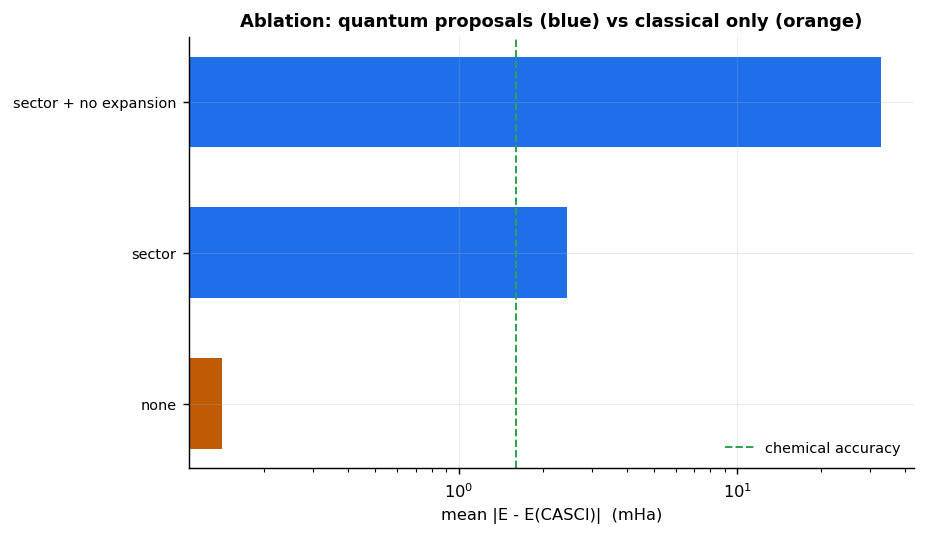
\includegraphics[width=0.60\textwidth]{figures/li2s-ablation.png}
\caption{The ablation, reproduced so that its negative reading is on the record.
The mean-error column of Table~\ref{tab:ablation} is not a like-for-like
comparison: the \code{sector} row averages fourteen runs including the two
\code{INCONSISTENT} geometries, while \code{none} is a single run at
equilibrium. The comparable figures are the ones at $2.10\Ang$ --- $0.1413\mHa$
classical against $0.0762\mHa$ quantum-sampled.}
\label{fig:ablation}
\end{figure}

\begin{caution}[Read the last column first]
The quantum sampler's measurable contribution is a \textbf{better starting
subspace}: first-iteration error $1.54\mHa$ classical against $2.23\mHa$
sampled over a set that includes the invalid geometries, and both converging to
comparable final energies at equilibrium. That is precisely what the method asks
of the circuit --- it proposes configurations, and the classical eigensolver
prices them. Where the final energies converge to the same place, the honest
statement is that \textbf{the classical expansion was sufficient for this system
at this size}, and this table is what makes that statement checkable rather than
assumed.
\end{caution}

Removing the classical half instead is decisive: sampling alone reaches only
$304$ determinants and $32.74\mHa$, and the run is additionally reported as
\code{SPIN CONTAMINATED}. The classical expansion is doing the majority of the
subspace construction at this scale.

\subsection{Classical baselines in the identical active space}

\begin{table}[htbp]
\centering
\caption{MP2, CCSD and CCSD(T) frozen to CAS(12e,12o), scored against the same
CASCI reference, with the $T_1$ diagnostic.}
\label{tab:classical}
\small
\begin{tabular}{rrrrr}
\toprule
$r$ (\AA) & MP2 err & CCSD err & CCSD(T) err & $T_1$ \\
\midrule
$1.700$ & $+7.11\mHa$  & $+2.95\mHa$  & $+0.31\mHa$  & $0.0239$ \\
$1.900$ & $+7.62\mHa$  & $+3.86\mHa$  & $+0.38\mHa$  & $0.0270$ \\
$2.000$ & $+7.85\mHa$  & $+4.29\mHa$  & $+0.40\mHa$  & $0.0287$ \\
$2.100$ & $+8.06\mHa$  & $+4.70\mHa$  & $+0.41\mHa$  & $0.0304$ \\
$2.200$ & $+8.25\mHa$  & $+5.08\mHa$  & $+0.41\mHa$  & $0.0321$ \\
$2.400$ & $+8.58\mHa$  & $+5.75\mHa$  & $+0.40\mHa$  & $0.0354$ \\
$2.600$ & $+8.93\mHa$  & $+6.34\mHa$  & $+0.41\mHa$  & $0.0387$ \\
$2.900$ & $+13.08\mHa$ & $+5.24\mHa$  & $+1.00\mHa$  & $0.0509$ \\
$3.200$ & $+16.80\mHa$ & $+5.88\mHa$  & $+1.54\mHa$  & $0.0625$ \\
$3.600$ & $+24.34\mHa$ & $+4.32\mHa$  & $+0.27\mHa$  & $0.0896$ \\
$4.200$ & $+68.50\mHa$ & $+34.37\mHa$ & $+29.83\mHa$ & $0.1134$ \\
$5.000$ & $+72.45\mHa$ & $+35.54\mHa$ & $+30.06\mHa$ & $0.1197$ \\
$6.000$ & $+59.30\mHa$ & $+35.67\mHa$ & $+29.48\mHa$ & $0.1216$ \\
\bottomrule
\end{tabular}
\end{table}

$T_1$ above roughly $0.02$ means the reference determinant no longer dominates,
so CCSD(T) stops being a gold standard there. Every geometry in this study is
already above that threshold, and by $4.20\Ang$, $T_1$ has reached $0.11$ and
CCSD(T) is $30\mHa$ from the reference where HI-VQE is $0.065\mHa$ from it.

That is the entire justification for the choice of reference. A study that used
CCSD(T) as its gold standard along this coordinate would report HI-VQE as
wrong by $30\mHa$ at long range, when what has happened is that the baseline
left its domain of validity.

\begin{caution}[The baselines beyond $4.20\Ang$ compare across spin sectors]
The classical methods are built on a closed-shell singlet reference determinant,
while the CASCI reference they are scored against returns a triplet beyond
$4.20\Ang$ (Table~\ref{tab:spin}). Part of the apparent $30\mHa$ failure is
therefore a singlet--triplet gap rather than a correlation error, and the two
contributions are not separated here. The $T_1$ argument above stands on its
own; the magnitude does not.
\end{caution}

\section{Discussion}

\subsection{What the instrumentation cost}

Three quantities were recorded beyond the energy: $\Ssq$ at the converged
subspace, the sign of the error against the reference, and the classical
ablation control. The first two are single expectation values on a state that is
already constructed. The third is one additional run per configuration, at
${\sim}3.7$ s per iteration --- cheaper than the runs it contextualises,
because it has no sampling step.

Against that cost, they produced: the identification of an invalid reference at
two geometries; the spin-sector transition along the coordinate, which reframes
the classical baselines' failure; and a bounded, checkable statement of what the
quantum layer contributed. None of the three would be recoverable from a result
file containing only energies.

\subsection{Where the cost actually is}

Measured at the real 24-qubit size, with a $20{,}000$-determinant subspace and
three iterations:

\begin{center}
\small
\begin{tabular}{lr}
\toprule
Setting & s / iteration \\
\midrule
default (SPSA every iteration)          & $16.0$ \\
\code{--optimizer-every 3}              & $11.1$ \\
\code{--optimizer none}                 & $\mathbf{6.2}$ \\
\code{--simulator none} (classical control) & $3.7$ \\
\code{--max-determinants 6000}          & $6.4$ \\
\bottomrule
\end{tabular}
\end{center}

\begin{result}[Shrinking the subspace is not a speed lever]
Going from $20{,}000$ determinants to $6{,}000$ saved nothing measurable and cost
$170\mHa$. The classical half of an iteration is dominated by fixed work ---
building the same-spin blocks, ranking expansion candidates --- and not by the
dimension. Lower \code{--max-determinants} when short of memory, never to save
time. What costs time is \textbf{sampling}, at roughly $2.5$ s per circuit
evaluation, and SPSA requests three of those per iteration instead of one.
\end{result}

\section{Claims not supported by these data}

\begin{enumerate}[leftmargin=1.4em,itemsep=0.3em]

\item \textbf{Quantum advantage, in any form.} The full space is $853{,}776$
  determinants and a laptop diagonalises it directly. Table~\ref{tab:ablation}
  shows a classical control matching the quantum-sampled run at equilibrium.

\item \textbf{That HI-VQE errs at $3.20$ and $3.60\Ang$.} The opposite:
  \S\ref{sec:invalid} argues the reference is wrong there. But neither is the
  HI-VQE energy at those points claimed as correct --- it is a lower number
  than a reference that is itself unreliable, and the correct action is to
  recompute the reference in the triplet sector, which was not done.

\item \textbf{The magnitude of the classical baselines' failure beyond
  $4.20\Ang$.} It mixes a correlation error with a singlet--triplet gap, and the
  two are not separated.

\item \textbf{A reproduction of the published total energies.} No geometry,
  per-point energies or orbital set are published for the reference study, so
  total energies are not reproducible. What is comparable is the error against
  each study's own CASCI and the determinant count.

\item \textbf{Anything about hardware.} All energies here are noiseless. Noise
  models and configuration recovery are implemented and available on the
  \code{aer} path, but no noisy production run is reported.

\item \textbf{That $2.3\%$ of the space is a general compression ratio.} It is
  the ratio at a $20{,}000$-determinant cap on this system. It is a consequence
  of the setting, not a discovered property.

\end{enumerate}

\section{Limitations}

\begin{enumerate}[leftmargin=1.4em,itemsep=0.2em]
\item One basis, one orbital set, one active space, one molecule.
\item The two invalid geometries were diagnosed but not repaired. Recomputing
  the reference in the correct spin sector at $3.20$ and $3.60\Ang$ would close
  the curve.
\item The ablation has one run per removed component against fourteen for the
  full method, so its mean-error column is not a like-for-like comparison; the
  per-geometry figures are.
\item Seed $1234$, $8192$ shots, single realisation. No statistics over sampling
  noise.
\item The classical baselines were computed with a closed-shell reference
  throughout, which is the subject of a caution above.
\end{enumerate}

\section{Conclusions}

\sloppy
\begin{enumerate}[leftmargin=1.4em,itemsep=0.25em]

\item HI-VQE reproduces exact diagonalisation of a $853{,}776$-determinant
  active space to better than $0.135\mHa$ at eleven of thirteen geometries,
  using a mean of $2.25\%$ of the determinant space and a single measurement
  setting in place of $15{,}697$ Pauli words.

\item The dissociation energy derived from that curve is within $0.051$
  kcal/mol of the exact value --- a stricter consistency test than any total
  energy, because the systematic error cancels in a difference.

\item At two geometries the method's variational bound was violated, which
  establishes that the reference and not the method is at fault. The
  non-monotonicity of the reference curve confirms it independently. A
  variationally bounded method is a free certificate on its own reference.

\item CCSD(T) leaves its domain of validity along this coordinate, diagnosably
  via $T_1$, which is why CASCI is the reference. A study using CCSD(T) as its
  gold standard would have mis-attributed a $30\mHa$ baseline failure to the
  quantum method.

\item The quantum sampler's contribution at this size is a better starting
  subspace, and the classical expansion is sufficient for the final energy. This
  is reported as measured, and the ablation is what makes it checkable.

\end{enumerate}
\fussy

\appendix

\section{Provenance digests}

\begin{center}
\small
\begin{tabular}{ll}
\toprule
Quantity & Digest (first 16 hex) \\
\midrule
Workflow (all runs)            & \code{172e18c7113058d6} \\
Cache, $r = 2.10\Ang$          & \code{0624b0292541bdb9} \\
Reference method               & CASCI, $\Ssq = 1.19\times10^{-14}$ \\
\bottomrule
\end{tabular}
\end{center}

Every cached Hamiltonian in \code{cache/} carries a matching
\code{.validated.json} receipt. The caches without a \code{(1)} suffix in the
external archive are superseded --- they precede a
\code{direct\_spin0} $\to$ \code{direct\_spin1} reference correction and differ
by $10.1\mHa$ in the CASCI energy at $6.00\Ang$ --- and no quantity in this
report uses them.

\section{Complete settings}

\begin{center}
\small
\begin{tabular}{ll}
\toprule
Setting & Value \\
\midrule
\code{--simulator}              & \code{sector} \\
\code{--max-determinants}       & $20{,}000$ \\
\code{--expansion}              & $400$ \\
\code{--expansion-references}   & $8$ \\
\code{--ranking}                & \code{pt2} \\
\code{--growth-factor}          & $3.0$ \\
\code{--amplitude-threshold}    & $10^{-6}$ \\
\code{--spin-complete}          & off \\
PT2 / \code{--pt2-factor}       & on / $4.0$ \\
\code{--max-iterations}         & $12$ \\
\code{--energy-tolerance}       & $10^{-6}\Ha$ \\
\code{--patience}               & $5$ \\
\code{--shots}                  & $8{,}192$ \\
\code{--init-scale}             & $0.4$ \\
\code{--optimizer}              & SPSA, 1 step, every iteration \\
\code{--seed}                   & $1234$ \\
Readout / depolarising error    & $0.0$ / $0.0$ \\
Configuration recovery          & enabled \\
\bottomrule
\end{tabular}
\end{center}

The paper's own selection rule is reproduced exactly by
\code{--expansion-references 1 --ranking coupling}; the default used here takes
the leading 8 configurations and ranks by the coherent first-order sum, which is
better informed. A \code{paper-rule} run at $2.10\Ang$ is included in the result
set for comparison and reaches $0.576\mHa$.

\section{Software environment}

Python 3.12.13, qiskit 2.5.2, qiskit-aer 0.17.2, NumPy 2.5.2, SciPy 1.18.0,
OpenFermion 1.8.1, matplotlib 3.11.1. PySCF 2.x on the machine that ran
\code{prepare}, \code{geometry} and \code{classical}; those three commands are
the only ones that require it.

\section{Reproduction}

\begin{verbatim}
python run.py selftest
python run.py backend --full

python run.py prepare  --all          # PySCF
python run.py classical --all         # PySCF

python run.py validate --all
python run.py scan
python run.py hivqe --distance 2.10 --simulator none      # ablation control
python run.py hivqe --distance 2.10 --no-expansion        # ablation control
python run.py report
\end{verbatim}

\code{colab.ipynb} performs the whole study, chemistry included, in one free
Colab session.

\section{Data inventory}

\begin{center}
\small
\begin{tabular}{ll}
\toprule
Path & Contents \\
\midrule
\code{cache/li2s\_r*.json}         & 13 cached Hamiltonians \\
\code{cache/li2s\_r*.validated.json} & their receipts \\
\code{results/hivqe\_r*\_sector.json} & 13 single-point runs \\
\code{results/hivqe\_r2.100\_none.json} & classical selected-CI control \\
\code{results/hivqe\_r2.100\_sector\_noexp.json} & sampler-only control \\
\code{results/hivqe\_r2.100\_sector\_paper-rule.json} & the paper's selection rule \\
\code{results/scan\_sector.json}   & the assembled dissociation scan \\
\code{results/classical.json}      & MP2 / CCSD / CCSD(T) ladder \\
\code{results/report.md}, \code{report.html} & the workflow's own report \\
\code{results/report\_data.json}   & every quantity behind it \\
\bottomrule
\end{tabular}
\end{center}

Sixteen single-point runs and one scan. Every quantity in this document is
recomputable from those files without re-running the algorithm.

\section*{References}
\small
\begin{enumerate}[leftmargin=1.4em,itemsep=0.1em]
\item M.\ Pellow-Jarman \emph{et al.} (Qunova Computing), \emph{Handover
  Iterative Variational Quantum Eigensolver}, arXiv:2503.06292 --- the method
  and the benchmark system reproduced here.
\item W.\ R.\ Clements \emph{et al.}, \emph{Optimal design for universal
  multiport interferometers}, Optica \textbf{3}, 1460 (2016) --- the
  decomposition that sets the required Givens network depth.
\item T.\ J.\ Lee and P.\ R.\ Taylor, \emph{Int.\ J.\ Quantum Chem.}
  \textbf{S23}, 199 (1989) --- the $T_1$ diagnostic of
  Table~\ref{tab:classical}.
\end{enumerate}

\end{document}
